\documentclass[10pt,twocolumn,letterpaper]{article}
\usepackage[review]{cvpr}
\usepackage{times}
\usepackage{graphicx}
\usepackage{amsmath,amssymb}
\usepackage{booktabs}
\usepackage{array,tabularx,multirow}
\usepackage{xcolor}
\usepackage{microtype}
\usepackage{tikz}
\usetikzlibrary{arrows.meta,positioning,calc,fit,shapes.geometric}
\usepackage{listings}
\usepackage{enumitem}
\usepackage{placeins}
\definecolor{atomblue}{HTML}{275D84}
\definecolor{atomteal}{HTML}{247B73}
\definecolor{atomgold}{HTML}{A16F20}
\definecolor{atomlight}{HTML}{F1F5F8}
\newcommand{\model}{\textsc{AtomVLA}}
\newcommand{\NE}{\textcolor{gray}{NE}}
\newcommand{\sg}{\operatorname{sg}}
\newcommand{\norm}[1]{\left\lVert#1\right\rVert}
\newcolumntype{Y}{>{\raggedright\arraybackslash}X}
\lstset{basicstyle=\ttfamily\footnotesize,columns=fullflexible,
  keepspaces=true,breaklines=true,frame=single,rulecolor=\color{gray!40},
  backgroundcolor=\color{atomlight},showstringspaces=false,
  aboveskip=6pt,belowskip=6pt}
\setlist[itemize]{leftmargin=*,nosep}
\setlist[enumerate]{leftmargin=*,nosep}

\usepackage{float}

\usepackage{cuted}
\raggedbottom

\definecolor{cvprblue}{rgb}{0.21,0.49,0.74}
\usepackage[pagebackref,breaklinks,colorlinks,allcolors=cvprblue]{hyperref}
\def\confName{CVPR}
\def\confYear{2027}

\title{AtomVLA: Atomic Programs as a Bridge between Semantics, Future State, and Action}
\author{Anonymous CVPR submission}

\begin{document}
\maketitle
\nolinenumbers

\begin{abstract}
Generalization and long-horizon manipulation remain challenging for embodied policies. Scaling pretraining and robot demonstrations expands behavioral coverage, but does not explicitly expose which physical operations can be shared across tasks. We investigate whether a reusable execution representation can reduce the need to relearn similar operations. We present \model{}, a vision-language-action framework built around typed atomic programs. Each call specifies an operation, object and target references, parameter slots, and a completion contract, separating reusable operation structure from execution details that must be grounded in the current scene. The text head generates the atomic name and string-valued arguments, while a program-conditioned action Query supplies only the terminal end-effector position and orientation. A future-imagination expert replaces an explicitly generated procedural body with an ordered sequence of intermediate and terminal visual predictions. An action expert uses these visual tokens, the Query, and robot state within concatenated mixture-of-transformers streams to generate continuous control. A code-data pipeline aligns discrete calls, terminal poses, future-image sequences, and demonstrated actions. We formulate matched evaluations of data efficiency, cross-context reuse, long-horizon composition, and physical execution, with component and feedback controls to test the proposed mechanisms. This proposal includes explicitly labeled planning estimates and synthetic feature visualizations; empirical validation remains pending.
\end{abstract}

\section{Introduction}
\label{sec:intro}

Embodied policies have made substantial progress, yet generalization and long-horizon manipulation remain challenging. Changes in objects, goals, viewpoints, or task composition can demand additional demonstrations or adaptation. A prominent response is to scale vision-language pretraining and robot demonstration data~\cite{rt1,rt2,palme,oxembodiment,octo,openvla,pi05,oft}. This broadens behavioral coverage, but leaves an important question: how can a policy reuse a learned physical operation when its context changes, rather than requiring separate examples for every combination of object, goal, and scene?

We hypothesize that an implicit execution interface contributes to this repeated learning. Many policies map observations and instructions to actions without explicitly identifying the active operation, its start and end boundaries, its completion condition, or the execution structure shared with other tasks. The same pick--move--place pattern may therefore appear in many demonstrations without an explicit unit through which to share it. Such an interface also makes long tasks harder to decompose and failures harder to localize. Our focus is \emph{data efficiency}: reducing the demonstrations needed to acquire transferable behavior. This is distinct from reducing inference latency or physical execution time, which must be measured separately.

Semantics provides a natural starting point for reuse, but does not determine physical execution. A \texttt{pick} operation retains its meaning across objects while requiring different contact regions, approach directions, end-effector poses, and trajectories. Likewise, ``place the object in the basket'' specifies a goal without fixing its motor realization. Stable semantics and variable execution details must therefore coexist in a useful primitive representation. Action-sequence policies~\cite{diffpolicy,act} model rich motor behavior, while multimodal prompting and hierarchical planning~\cite{vima,saycan,progprompt,inner} expose task structure; the remaining challenge is to connect reusable operation structure to scene-specific control.

An atomic execution representation should expose five properties: stable operation semantics, explicit boundaries and completion contracts, references to current objects and targets, a separation between reusable structure and geometric details, and a mechanism for recovering those details from the current observation. Typed program calls provide a concrete way to express this interface. A call names an operation, declares its reference and parameter slots, and specifies when execution is complete. Its schema can be checked and composed with other calls; the concrete object bindings and continuous values are resolved anew in each scene. The reusable element is the operation and its typed argument/contract structure, not a fixed object identity or trajectory.

\begin{figure*}[t]
\centering
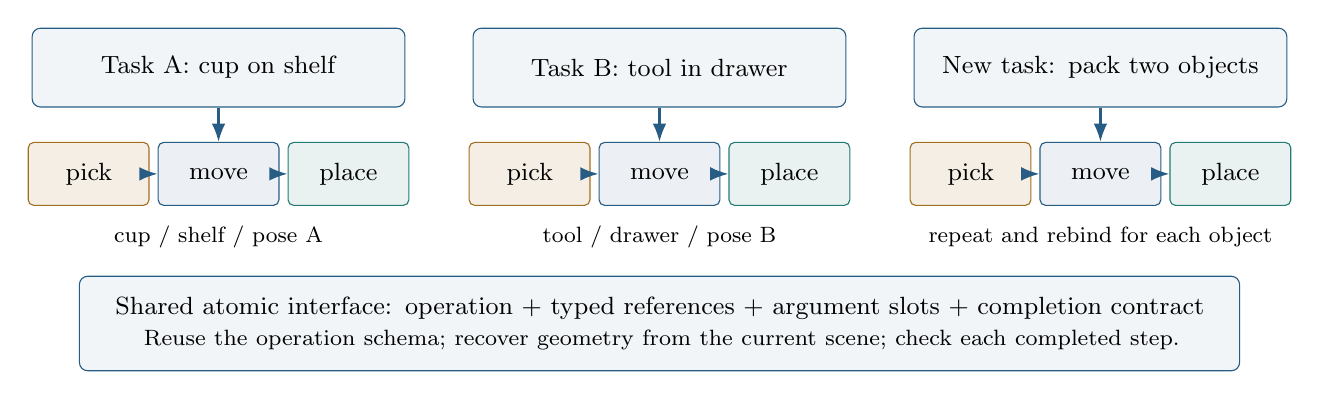
\begin{tikzpicture}[>=Latex,font=\small,
 task/.style={draw=atomblue,fill=atomlight,rounded corners=3pt,align=center,text width=45mm,minimum height=10mm},
 pick/.style={draw=atomgold,fill=atomgold!12,rounded corners=2pt,align=center,text width=13mm,minimum height=8mm},
 move/.style={pick,draw=atomblue,fill=atomblue!9},
 place/.style={pick,draw=atomteal,fill=atomteal!10},
 arr/.style={->,thick,draw=atomblue}]
\node[task] (a) at (0,0) {Task A: cup on shelf};
\node[task] (b) at (5.6,0) {Task B: tool in drawer};
\node[task] (c) at (11.2,0) {New task: pack two objects};
\node[pick] (a1) at (-1.65,-1.35) {pick};
\node[move] (a2) at (0,-1.35) {move};
\node[place] (a3) at (1.65,-1.35) {place};
\node[pick] (b1) at (3.95,-1.35) {pick};
\node[move] (b2) at (5.6,-1.35) {move};
\node[place] (b3) at (7.25,-1.35) {place};
\node[pick] (c1) at (9.55,-1.35) {pick};
\node[move] (c2) at (11.2,-1.35) {move};
\node[place] (c3) at (12.85,-1.35) {place};
\foreach \x/\y in {a1/a2,a2/a3,b1/b2,b2/b3,c1/c2,c2/c3}{\draw[arr] (\x)--(\y);}
\draw[arr] (a)--(a2);\draw[arr] (b)--(b2);\draw[arr] (c)--(c2);
\node[align=center,font=\footnotesize] at (0,-2.15) {cup / shelf / pose A};
\node[align=center,font=\footnotesize] at (5.6,-2.15) {tool / drawer / pose B};
\node[align=center,font=\footnotesize] at (11.2,-2.15) {repeat and rebind for each object};
\node[task,text width=145mm,minimum height=12mm] (shared) at (5.6,-3.25)
{Shared atomic interface: operation + typed references + argument slots + completion contract\\
\footnotesize Reuse the operation schema; recover geometry from the current scene; check each completed step.};
\end{tikzpicture}
\caption{\textbf{Why atomic actions matter.} Tasks with different objects and goals share physical operations. Typed atoms expose reusable boundaries and contracts while scene-specific references and geometry change. Rebinding and composing familiar calls supports new task sequences and localizes failed steps, instead of requiring an independent representation for every whole-task variation. These are the proposed mechanisms, not measured efficiency gains.}
\label{fig:motivation}
\end{figure*}

Programs provide structure, but symbols alone do not provide grounding. Reusing the same \texttt{pick} or \texttt{place} call still requires estimating a physically appropriate future configuration from the current scene. Program-based control~\cite{codeaspolicies,progprompt,aw0} motivates an inspectable intermediate interface, while representations of physical semantics and state transitions~\cite{physicalwords,vladelta} motivate grounding that interface in its expected outcome. We combine these ideas by separating the discrete call, its terminal geometry, and its imagined visual evolution. A typed call is a structured intent interface; it need not contain an executable function body.

We propose \model{}, in which the text branch generates an atomic name and string-valued arguments, and a \emph{program-conditioned action Query} supplies the continuous parameters: terminal end-effector position and orientation. Query predicts only this endpoint, not a sequence of intermediate poses. To represent what happens within the primitive, a future-imagination expert generates a primitive-dependent sequence of event keyframes conditioned on the current scene, the call, and terminal geometry. This learned evolution replaces an explicitly generated procedural body. For example, a pick may be represented by imagined pregrasp, closure, and lift keyframes rather than generated control statements.

The action expert reads the shared Query, robot state, and imagined visual tokens to generate continuous actions. Image and action tokens remain concatenated within a mixture-of-transformers (MoT) and jointly denoise through modality-specific experts. Thus imagined visual evolution supplies intermediate context, while the action expert learns timing, contact adjustments, and gripper control. Neither a plausible image sequence nor an accurate endpoint guarantees successful execution.

Our code-data pipeline binds each discrete call to synchronized current observations, robot state, one completion pose per active arm, an ordered future-image sequence, and demonstrated actions. Following prior robot data engines~\cite{robomimic,mimicgen,oxembodiment}, it records boundaries, timestamps, coordinate frames, and validity masks. Future frames supervise imagination during training and are never inference inputs. At runtime, the policy executes a short action prefix, observes the result, and regenerates the remaining evolution or advances according to the observed completion condition.

The resulting hypothesis is that explicit reusable structure, coupled with scene-dependent geometric grounding, can improve transfer and composition with fewer demonstrations. This benefit is not guaranteed by program syntax or pose prediction alone. We test it through matched data-budget comparisons, held-out contexts, component ablations, memory interventions, and planner--controller feedback controls. Task success remains the primary outcome; intermediate prediction accuracy and feature clustering are supporting measurements.

Our contributions are:
\begin{itemize}
\item a typed atomic-program interface that separates reusable operation structure from scene-specific execution details, targeting cross-context reuse and long-horizon composition;
\item a code-data pipeline aligning each call with current observations, terminal poses, ordered future-image sequences, and demonstrated actions;
\item a terminal-pose action Query and future imagination that separate endpoint grounding from within-primitive visual evolution, conditioning continuous control through concatenated image/action MoT experts;
\item a matched evaluation protocol for data efficiency, primitive reuse, multimodal conditioning, and physical execution, with controls that distinguish architectural hypotheses from measured benefits.
\end{itemize}
\section{Related Work}
\label{sec:related}
\textbf{Vision-language-action policies.} RT-1 and RT-2 connect visual-language pretraining to robot control, while PaLM-E and Open X-Embodiment broaden embodied inputs and demonstration coverage~\cite{rt1,rt2,palme,oxembodiment}. Octo, OpenVLA, $\pi_{0.5}$, and OpenVLA-OFT study generalist control, transfer, and efficient action adaptation~\cite{octo,openvla,pi05,oft}. Diffusion Policy and ACT capture fine-grained behavior through continuous action sequences~\cite{diffpolicy,act}. These advances improve the learned policy but do not inherently expose a reusable, checkable operation boundary. AtomVLA retains a continuous action expert and studies whether explicit primitive structure can reduce repeated learning across objects, goals, and task compositions. This representation question complements scaling rather than assuming that program syntax alone solves generalization.

\textbf{Programs and physical semantics.} Code as Policies, ProgPrompt, and SayCan use programs or situated plans to organize behavior~\cite{codeaspolicies,progprompt,saycan}. Physical Words aligns physical semantics with future sensory dynamics, VLA-$\Delta$ models state transitions, and LexiconVLA explores atomic codebooks~\cite{physicalwords,vladelta,lexiconvla}. AW-0 jointly models code, future video, and actions through a multimodal expert framework~\cite{aw0}. Our program vocabulary follows Physical Words, while each typed call additionally exposes references, continuous argument slots, and a completion contract. The text branch predicts discrete names and string arguments; a completion-pose Query supplies continuous terminal geometry. Future imagination replaces an explicitly generated function body with ordered visual predictions, and the concatenated action expert uses those tokens for continuous control. The distinction concerns how programs acquire instance-specific geometry and condition execution, not the mere presence of code or multiple output modalities.

\textbf{Hierarchy, memory, and robot data.} Language hierarchies, embodied reasoning, visual goals, and interactive feedback offer mechanisms for long-horizon manipulation~\cite{rth,ecot,cotvla,inner}. RMBench further emphasizes tasks whose solution depends on retaining historical state~\cite{chen2026rmbench}. RoboMimic, MimicGen, and Open X-Embodiment support standardized trajectories, scalable demonstration generation, and cross-context reuse~\cite{robomimic,mimicgen,oxembodiment}. AtomVLA connects these themes through a primitive-level annotation pipeline: each interval receives a typed call, a verified completion event, a terminal pose and synchronized multi-frame RGB targets, and an action chunk. Completion contracts also provide explicit update points for the optional memory and feedback interfaces. We evaluate these extensions with reset, shuffled-history, and feedback controls so that their benefits are not inferred from hierarchy or clustering alone. Additional discussion appears in Appendix~\ref{app:related}.

\section{Method}
\label{sec:method}
AtomVLA separates atomic execution into discrete intent, terminal geometry, and imagined evolution. A text head generates the atomic name and string-valued arguments; action Query supplies only the terminal end-effector pose. A future-imagination expert models the intermediate visual evolution that would otherwise be specified by a primitive's procedural body, and an action expert generates executable control. Figure~\ref{fig:overview} shows their shared MoT interface.

\begin{figure*}[t]
\centering
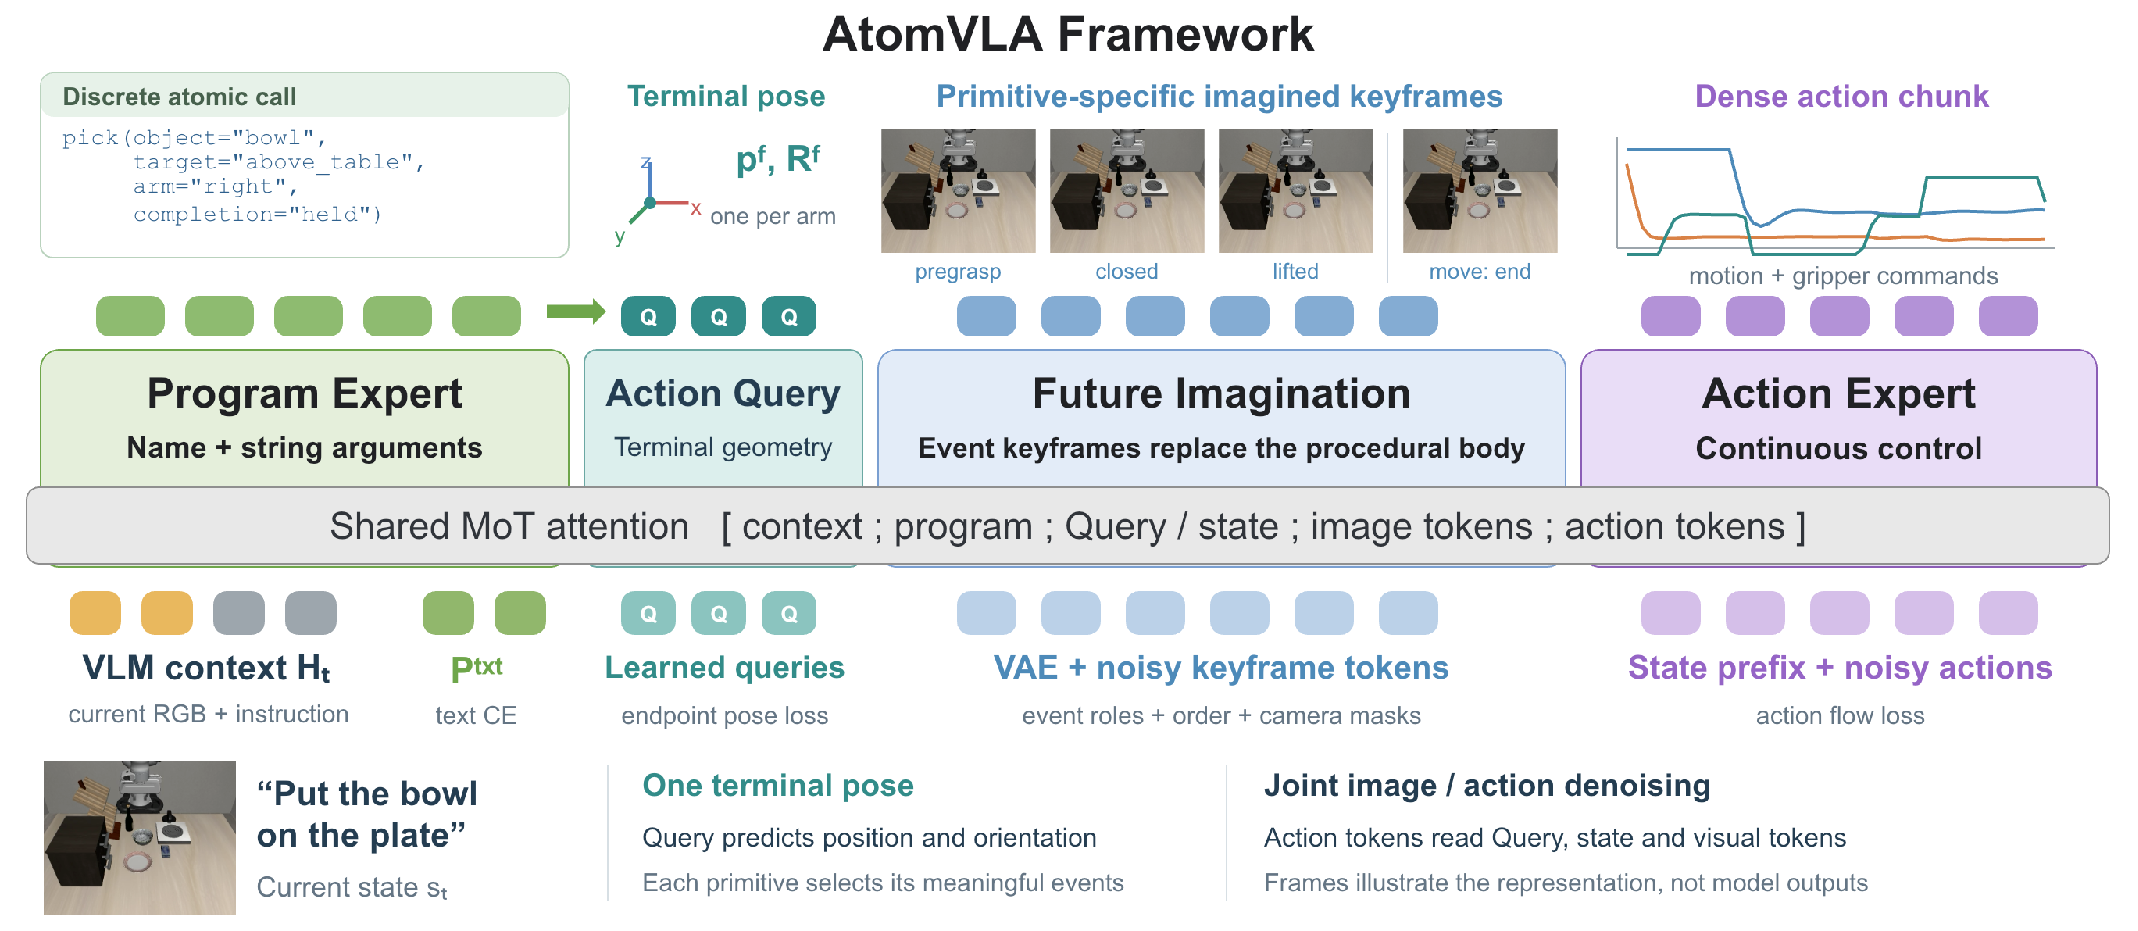
\includegraphics[width=\textwidth]{atomvla_framework.pdf}
\caption{\textbf{AtomVLA architecture.} The program expert emits an atomic name and string arguments. Action Query predicts only the terminal position and orientation per active arm. Future imagination represents within-primitive evolution as ordered visual states, replacing a generated executable function body. Concatenated image/action streams jointly denoise through MoT attention; action tokens read Query, robot state, and evolving visual tokens. Pick illustrates pregrasp, closure, and lift; move illustrates arrival. These are demonstration examples of different event structures, not measured predictions.}
\label{fig:overview}
\end{figure*}

\subsection{Dataset Annotation Pipeline}
\label{sec:data}
We align each demonstrated primitive with a discrete call, one terminal pose per active arm, an ordered future-image sequence, and action chunks. The call names an operation and uses strings for object, target, arm, contact mode, and completion condition. Only position and orientation are continuous call parameters; they are supervised separately through action Query. No executable function body is a prediction target. The semantic vocabulary follows the 16 Physical Words labels~\cite{physicalwords}; schemas and coverage conventions appear in Appendix~\ref{app:vocabulary}.

\begin{figure*}[t]
\centering
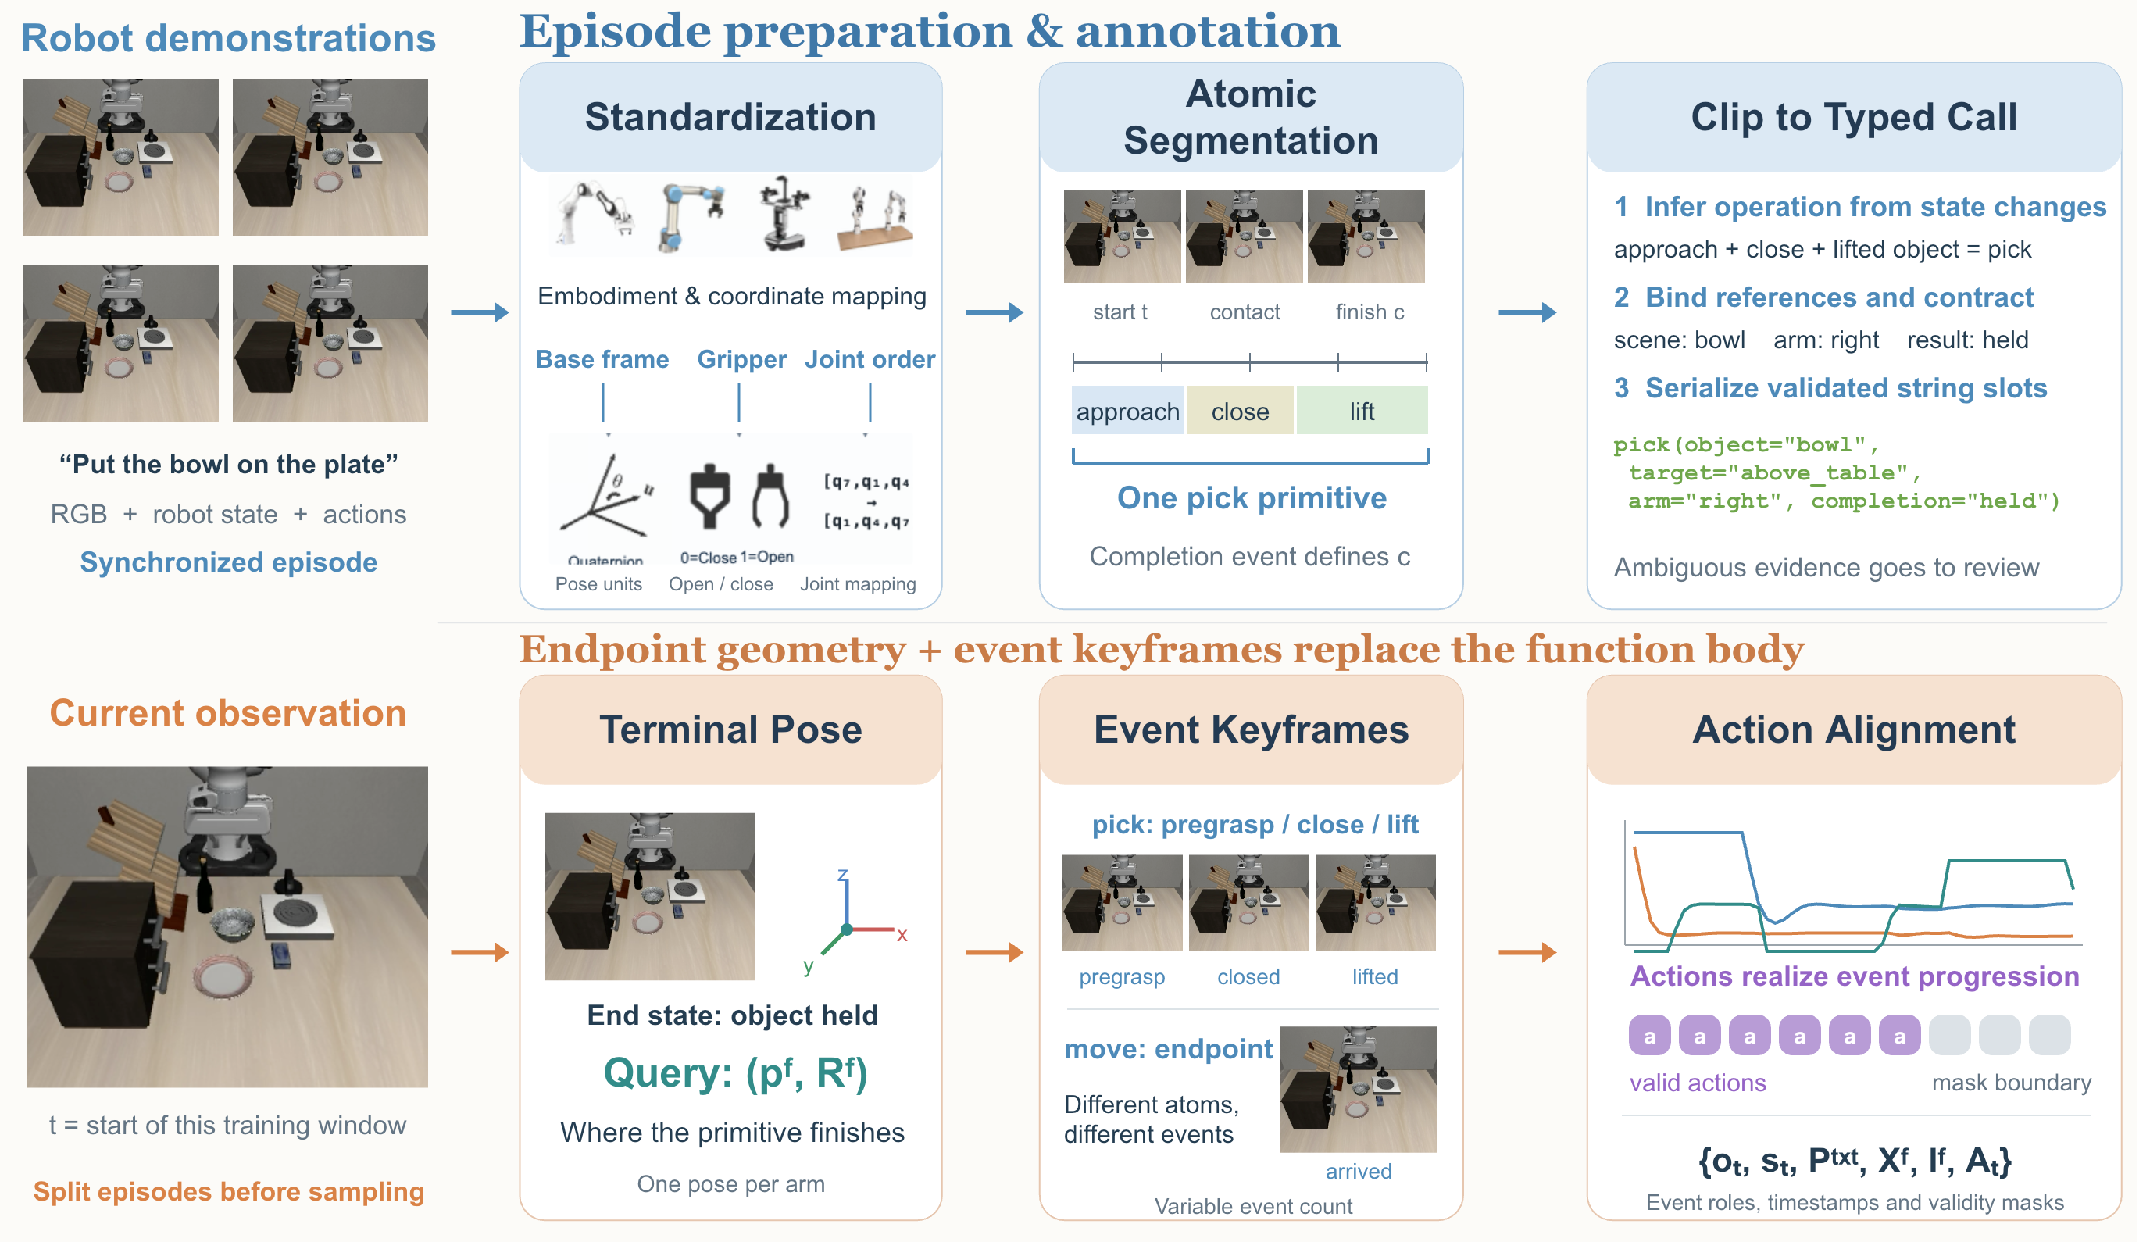
\includegraphics[width=\textwidth]{atomvla_annotation_pipeline.pdf}
\caption{\textbf{Dataset annotation pipeline.} The upper row standardizes synchronized demonstrations, identifies primitive intervals, then infers verbs from observed state changes, binds scene references, checks contracts, and serializes typed calls. The lower row aligns the current observation with a terminal pose, primitive-specific event frames, and demonstrated actions. Endpoint geometry and imagined events jointly replace the procedural body. The LIBERO images illustrate one pick interval within a bowl-placement episode; these are source demonstration frames, not model predictions.}
\label{fig:annotation}
\end{figure*}

\textbf{Clip-to-program conversion.} After synchronization and segmentation, we infer each operation from its observed state changes, ground object/target references in the scene, assign the arm, and check the completion contract. Approach, closure, and an object moving with the gripper support a single \texttt{pick} call. We serialize validated names and string slots; continuous terminal geometry remains a separate target. Ambiguous bindings, unverified events, and failed attempts enter review rather than acquiring successful labels.

\textbf{Multimodal target alignment.} For current time $t$ and verified completion $c(t)$, $X_t^F$ contains the terminal end-effector position and orientation. The call and observed phase determine meaningful event roles: \texttt{pick} uses pregrasp, closure, and lift, whereas a simple \texttt{move} can use arrival alone. Verified events give $t<\tau_1<\cdots<\tau_{K_i}=c(t)$ and $\mathcal I_t^F=(o_{\tau_1},\ldots,o_{\tau_{K_i}})$, with variable $K_i$ rather than uniform temporal sampling. A record is
\begin{equation}
\mathcal D_i=(o_t,l,s_t,P_t^{\rm txt},X_t^F,\mathcal I_t^F,A_t,\mu_i).
\label{eq:record}
\end{equation}
Metadata records timestamps, frames, arm/camera masks, and annotation quality. Both arms and all available cameras share the same temporal indices. Action chunks are truncated or masked at boundaries; invalid or failed outcomes receive no invented successful targets. Appendix~\ref{app:annotation} details temporal sampling and quality checks.

\subsection{Model and Training}
\label{sec:program}
\textbf{Discrete call and terminal Query.} The VLM encodes current inputs as $H_t$. Its text head predicts $P_t^{\rm txt}=(v_t,r_t,d_t,\kappa_t)$: the operation name, object/target references, other string arguments, and a string-valued completion condition. It generates neither numeric pose tokens nor function bodies. Learned Query tokens ground the terminal geometry:
\begin{equation}
Q_t=\operatorname{Query}(H_t,E_P(P_t^{\rm txt}),s_t),\quad
\widehat X_t^F=D_{\rm pose}(Q_t).
\label{eq:query}
\end{equation}
\label{sec:query}
The call's continuous parameters are the predicted terminal position and orientation in a calibrated robot-base frame, one pose per valid arm. Query does not predict intermediate waypoints, RGB, or motor commands. Its latent tokens and decoded terminal pose condition the downstream experts. Position and geodesic rotation losses supervise this endpoint without assuming that endpoint accuracy determines the path.

\textbf{Future imagination in MoT.}
\label{sec:mot}
The image expert predicts $\widehat{\mathcal I}_t^F$ from current context, the call, and terminal geometry. Pose specifies where the primitive finishes; imagined keyframes express its internal event progression. For \texttt{pick}, they describe pregrasp, closure, and lift. A simple \texttt{move} may require only arrival; contact or obstacle negotiation can require additional reviewed event schemas. Thus internal logic becomes a learned visual representation whose content and length depend on the primitive. The action expert realizes the dense motion between these states.

Image and action experts retain the concatenated MoT structure:
\begin{equation}
\begin{aligned}
C_t&=[H_t;E_P(P_t^{\rm txt});E_s(s_t);Q_t;E_X(\widehat X_t^F)],\\
Z_\sigma&=[C_t;E_I(\mathcal I_{t,\sigma}^F);E_A(A_{t,\sigma})].
\end{aligned}
\label{eq:motconcat}
\end{equation}
Event-role, order, and camera embeddings distinguish keyframes; padding carries no loss. At runtime, remaining roles follow the call schema and phase inferred from observations, never future annotations. The action stream attends to the evolving image tokens, together with Query and current state, to generate dense action chunks including gripper commands. Image/action tokens jointly denoise through modality-specific experts; the diagram's semantic dependence does not require a separate image-only rollout before every action. Clean future frames are never inference inputs, and current-context tokens cannot read future-target tokens. Appendix~\ref{app:losses} specifies the generation mask and losses.

\textbf{Training.} Warm-up trains the text head and Query/pose modules on aligned records with pretrained backbones frozen. Text cross-entropy supervises only the discrete call; all continuous call parameters are learned through terminal-pose supervision. Joint training then updates these modules, the image/action experts, and selected backbone adapters. Sequence RGB supervision teaches the imagined intermediate evolution, while demonstrated actions supervise physical control:
\begin{equation}
\mathcal L=\mathcal L_{\rm txt}+\lambda_p\mathcal L_{\rm pose}
+\lambda_i\mathcal L_{\rm seq}+\lambda_a\mathcal L_{\rm act}.
\label{eq:training}
\end{equation}
Losses use valid-target masks. Image and action losses also update the shared representation; the pose head receives no intermediate-waypoint regression objective. Joint batches mix annotated and decoded discrete calls, but downstream geometric conditioning always uses predicted Query outputs. Details and fixed-before-evaluation defaults appear in Appendix~\ref{app:training}.

\textbf{Closed-loop execution.} The model generates a discrete call, predicts its terminal pose, and imagines the within-primitive visual evolution while synthesizing actions. It executes a short action prefix, obtains new observations, and regenerates the remaining predictions. Observed completion advances to the next call; unmet conditions permit continued execution or re-grounding. Imagination is a learned forecast, not a correctness guarantee or a simulator. The action expert realizes motion and contact; robot-specific controllers execute its actions. Optional memory and feedback remain separately evaluated extensions.

\section{Experiments}
\label{sec:experiments}
\paragraph{Benchmarks.}
We use LIBERO~\cite{libero} for generalization, LIBERO-Pro~\cite{liberopro} for robustness, RoboTwin~2.0~\cite{robotwin} for dual-arm manipulation, and RoboMME~\cite{robomme} for memory-dependent behavior. Five distinct real-robot tasks additionally test articulated, contact-rich, and deformable-object manipulation. LIBERO uses an overall average, LIBERO-Pro retains its five perturbation subsets, and RoboTwin reports Easy and Hard settings.

\paragraph{Baselines.}
We compare $\pi_{0.5}$, OpenVLA-OFT, VLA-$\Delta$, Physical Words, AW-0, and LexiconVLA~\cite{pi05,oft,vladelta,physicalwords,aw0,lexiconvla}. The RoboMME study compares general-purpose policies and a matched text-conditioned controller, rather than specialized memory architectures. The component and controller studies share three RoboTwin tasks: Handover Block, Place Object Basket, and Put Bottles Dustbin.

\paragraph{Report status.}
All projected scores, including comparator values, are planning estimates; the feature plot is synthetic. Published references are marked separately. Each experiment specifies its purpose and procedure, expected pattern, and conditional interpretation. Full settings and statistical tests are in Appendix~\ref{app:experiments}.

\subsection{Benchmark Performance}
\label{sec:benchmarks}
\textbf{Purpose and procedure.} We test whether reusable programs and pose grounding transfer beyond nominal training conditions. Policies use matched demonstration identities and budgets, then run on the same LIBERO, LIBERO-Pro, and RoboTwin evaluation manifests. LIBERO-Pro changes object attributes, initial positions, instruction phrasing, task goals, and environments. Nested demonstration budgets and held-out primitive compositions separately test data efficiency and reuse. Table~\ref{tab:liberopro} gives the expected benchmark scenario.

\begin{table*}[t]
\centering
\footnotesize
\setlength{\tabcolsep}{2.5pt}
\caption{\textbf{Benchmark planning estimates (\%).} All scores are projected, including baselines. LIBERO-Pro averages five perturbations. -- indicates an unplanned evaluation.}
\label{tab:liberopro}
\resizebox{\textwidth}{!}{%
\begin{tabular}{@{}l c *{7}{c} *{2}{c}@{}}
\toprule
& LIBERO & \multicolumn{7}{c}{LIBERO-Pro} & \multicolumn{2}{c}{RoboTwin 2.0}\\
\cmidrule(lr){2-2}\cmidrule(lr){3-9}\cmidrule(lr){10-11}
Method & Average & Unperturbed & \shortstack{Object\\attributes} & \shortstack{Initial\\positions} & \shortstack{Semantic\\paraphrase} & \shortstack{Task-goal\\changes} & \shortstack{Environment\\replacement} & Average & Easy & Hard\\
\midrule
$\pi_{0.5}$~\cite{pi05} & 91.7 & 90.7 & 75.5 & 70.9 & 81.2 & 60.6 & 58.3 & 69.3 & 72.6 & 44.6 \\
OpenVLA-OFT~\cite{oft} & 90.8 & 89.5 & 73.2 & 67.3 & 79.8 & 55.6 & 54.5 & 66.1 & 64.3 & 38.4 \\
VLA-$\Delta$~\cite{vladelta} & 93.1 & 92.8 & 80.9 & 77.3 & 84.2 & 66.2 & 63.2 & 74.4 & 75.4 & 52.1 \\
PhysWord~\cite{physicalwords} & 90.1 & 89.4 & 77.6 & 73.6 & 83.8 & 63.6 & 60.6 & 71.8 & -- & --\\
AW-0~\cite{aw0} & 94.2 & 93.9 & 84.7 & 80.1 & 87.6 & 72.5 & 70.9 & 79.2 & 80.2 & 57.5 \\
LexiconVLA~\cite{lexiconvla} & 91.9 & 90.4 & 80.4 & 76.5 & 84.6 & 67.9 & 64.1 & 74.7 & -- & --\\
\model{} (ours) & 96.3 & 93.1 & 85.4 & 81.8 & 87.7 & 76.7 & 73.7 & 81.1 & 91.4 & 78.2 \\
\bottomrule
\end{tabular}}
\end{table*}

\textbf{Expected results and interpretation.} The revised AtomVLA scenario reaches 96.3\% on LIBERO and 91.4/78.2\% on RoboTwin Easy/Hard, matching the project's updated performance targets. The LIBERO-Pro scenario remains 81.1\%; its comparator values are planning assumptions, not verified public results. Consequently, this table does not establish a published leaderboard ranking. Matched evaluations must test whether typed operation reuse and scene-dependent pose grounding produce these gains. Data efficiency further requires the planned success-versus-budget comparison.

\subsection{Component Ablations}
\label{sec:ablations}
\textbf{Purpose and procedure.} We isolate the typed program, terminal-pose Query, future-imagination stream, and discrete program arguments on the three RoboTwin tasks. Full, no-program, no-Query, no-RGB, and verb-only variants share observations, action targets, data splits, and training budgets. Additional program-mask and pose-loss-off controls distinguish semantics from interface and supervision effects. Table~\ref{tab:ablation} reports the central planning scenario.

\begin{table}[H]
\centering\footnotesize
\setlength{\tabcolsep}{2pt}
\caption{\textbf{Component planning estimates (\%).} Matched RoboTwin tasks. All entries are projected.}
\label{tab:ablation}
\begin{tabularx}{\columnwidth}{@{}Yccc@{}}
\toprule
Variant & \shortstack{Handover\\Block} $\uparrow$ & \shortstack{Place Object\\Basket} $\uparrow$ & \shortstack{Put Bottles\\Dustbin} $\uparrow$\\
\midrule
Full \model{} & 47.1 & 70.9 & 58.8 \\
No program & 27.1 & 53.2 & 35.9 \\
No Query & 33.9 & 57.9 & 41.2 \\
No RGB generation & 45.3 & 68.9 & 55.8 \\
Verb-only program & 30.9 & 49.3 & 33.2 \\
\bottomrule
\end{tabularx}
\end{table}

\textbf{Expected results and interpretation.} Across the three tasks, Full averages 58.9\%, versus 38.7\% without a program, 44.3\% without Query, 56.7\% without RGB generation, and 37.8\% with verbs only. The assumed pattern assigns a larger contribution to program/geometry binding than to RGB supervision. If confirmed under the additional controls, it would support typed arguments and pose grounding as useful components; the small RGB gap would motivate assessing multi-frame imagination against a terminal-image-only control and its compute cost. These means summarize estimates, not ablation measurements.

\subsection{History-Dependent Tasks}
\label{sec:memory}
\textbf{Purpose and procedure.} We use RoboMME~\cite{robomme} as a stress test of history-dependent execution, rather than a benchmark for a new memory architecture. Its 16 tasks cover Counting, Permanence, Reference, and Imitation. Table~\ref{tab:memory} compares general-purpose $\pi_{0.5}$, its past-action variant, a matched text-conditioned controller, and AtomVLA. The matched controllers receive the same observed-history budget; AtomVLA carries program and completion context between primitives. Reset and shuffled-history controls test whether useful past information contributes beyond current-frame control. Settings are in Appendix~\ref{app:memory}.

\begin{table*}[t]
\centering
\scriptsize
\setlength{\tabcolsep}{2pt}
\renewcommand{\arraystretch}{1.15}
\caption{\textbf{General-policy comparison on RoboMME (\%, higher is better).} Columns follow RoboMME Table~3~\cite{robomme}. The two $\pi_{0.5}$ rows are published results; the matched text-control and AtomVLA rows are planning estimates, not measurements. AVG averages all 16 tasks.}
\label{tab:memory}
\resizebox{\textwidth}{!}{%
\begin{tabular}{@{}l*{17}{c}@{}}
\toprule
& \multicolumn{4}{c}{Counting} & \multicolumn{4}{c}{Permanence} & \multicolumn{4}{c}{Reference} & \multicolumn{4}{c}{Imitation} & \\
\cmidrule(lr){2-5}\cmidrule(lr){6-9}\cmidrule(lr){10-13}\cmidrule(lr){14-17}
Method & \shortstack{Bin\\Fill} & \shortstack{Pick\\Xtimes} & \shortstack{Swing\\Xtimes} & \shortstack{Stop\\Cube} & \shortstack{Video\\Umsk} & \shortstack{Button\\Umsk} & \shortstack{Video\\UmskS} & \shortstack{Button\\UmskS} & \shortstack{Pick\\HighL} & \shortstack{Video\\Repick} & \shortstack{Video\\PlcBtn} & \shortstack{Video\\PlcOrd} & \shortstack{Move\\Cube} & \shortstack{Insert\\Peg} & \shortstack{Pattern\\Lock} & \shortstack{Route\\Stick} & AVG\\
\midrule
$\pi_{0.5}$ & 30.00 & 42.89 & 35.56 & 6.67 & 20.44 & 22.22 & 18.67 & 6.67 & 11.33 & 0.44 & 31.11 & 25.78 & 26.00 & 1.56 & 2.89 & 4.67 & 17.93 \\
$\pi_{0.5}$ + past actions & 26.67 & 58.33 & 26.67 & 4.67 & 30.67 & 23.67 & 20.67 & 16.00 & 12.33 & 8.67 & 24.00 & 18.67 & 34.00 & 1.00 & 4.00 & 5.67 & 19.73 \\
Planner + text-loss & 43.7 & 71.6 & 63.8 & 24.5 & 53.2 & 45.7 & 32.4 & 22.6 & 42.9 & 27.3 & 49.8 & 31.7 & 65.4 & 10.6 & 36.2 & 42.8 & 41.5 \\
\model{} & 68.3 & 91.7 & 86.2 & 36.8 & 79.4 & 67.6 & 51.3 & 34.9 & 64.7 & 45.8 & 67.2 & 49.6 & 88.1 & 18.7 & 61.4 & 69.3 & 61.3 \\
\bottomrule
\end{tabular}}
\end{table*}

\textbf{Expected results and interpretation.} The planning scenario averages 61.3\% for AtomVLA and 41.5\% for the matched text-conditioned controller. The published $\pi_{0.5}$ and past-action averages are 17.93\% and 19.73\%, respectively; these provide context rather than a matched reproduction. The hypothesis is that typed calls and completion context support event tracking and object binding while future imagination supports execution. InsertPeg and StopCube remain difficult. The estimated gap is not empirical evidence: general-policy gains must hold under matched inputs, training, and history budgets, and reset/shuffled-history controls must establish any contribution from retained history. This study does not claim superiority over specialized memory systems.

\subsection{Controller Feedback}
\label{sec:coupling}
\textbf{Purpose and procedure.} We test whether the planner--controller interface supports recovery after execution deviations. Table~\ref{tab:coupling} compares direct action generation, planner+$\pi_{0.5}$, text-loss conditioning, and AtomVLA on the same three RoboTwin tasks. For causal analysis, the same AtomVLA checkpoint also runs with feedback off, valid feedback, and shuffled feedback under equal retry budgets. Completion-time pose discrepancy and observed contract status define the feedback signal.

\begin{table}[H]
\centering\footnotesize
\setlength{\tabcolsep}{2pt}
\caption{\textbf{Controller planning estimates (\%).} All entries are projected. AtomVLA matches Full in Table~\ref{tab:ablation}.}
\label{tab:coupling}
\begin{tabularx}{\columnwidth}{@{}Yccc@{}}
\toprule
Architecture & \shortstack{Handover\\Block} $\uparrow$ & \shortstack{Place Object\\Basket} $\uparrow$ & \shortstack{Put Bottles\\Dustbin} $\uparrow$\\
\midrule
Single VLM action model & 19.8 & 38.2 & 24.9 \\
Planner + $\pi_{0.5}$ & 18.8 & 48.4 & 30.7 \\
Planner + text-loss & 30.3 & 54.6 & 37.4 \\
Planner + \model{} & 47.1 & 70.9 & 58.8 \\
\bottomrule
\end{tabularx}
\end{table}

\textbf{Expected results and interpretation.} The planner--controller scenario averages 58.9\% for AtomVLA, versus 40.8\% for text-loss conditioning and 32.6\% for planner+$\pi_{0.5}$: gains of 18.1 and 26.3 percentage points. On the three tasks, the gains over text conditioning are 16.8, 16.3, and 21.4 points. This comparison tests whether the planning brain's typed intent and the control module's continuous execution cooperate through a shared geometric Query. These task-specific estimates are distinct from the full-suite Easy/Hard averages in Table~\ref{tab:liberopro}. Architecture-level gains do not isolate feedback: correction utility requires valid feedback to outperform off and shuffled feedback at equal retry budgets.

\subsection{Feature Structure}
\label{sec:representation}
\textbf{Purpose and procedure.} We examine whether typed programs with Query preserve action semantics across contexts. The eventual analysis extracts the same held-out primitive samples at a common layer and pooling rule, then fits a shared PCA projection for Text and Program+Query. The present two-panel illustration uses the 16-label Physical Words vocabulary with 6,400 synthetic points per panel and retains partial overlap.

\begin{figure}[H]
\centering
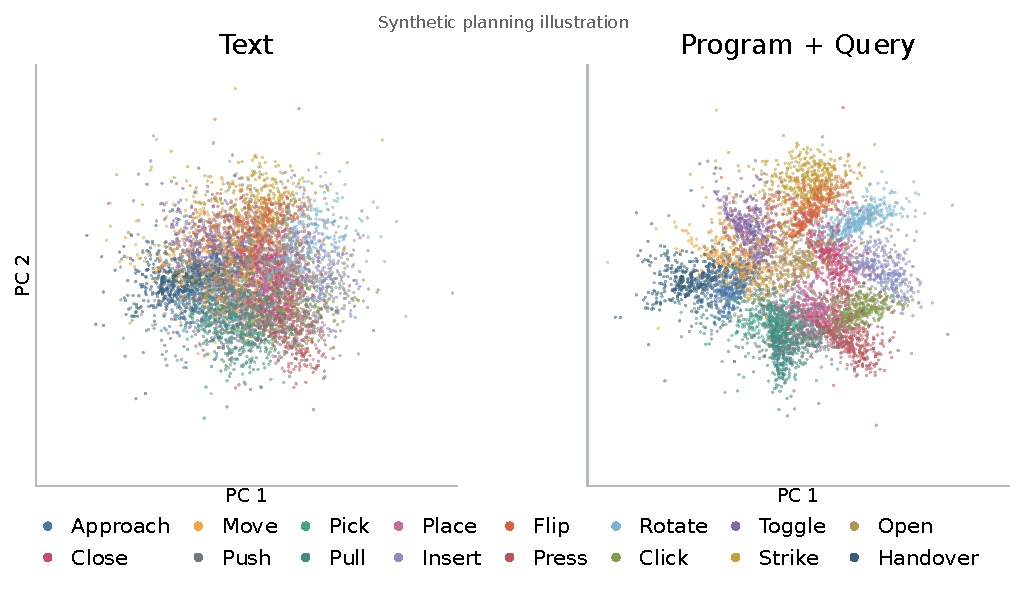
\includegraphics[width=\columnwidth]{expected_feature_comparison.pdf}
\caption{\textbf{Synthetic expected features.} Text and Program+Query share a PCA projection of generated 64-D features, with 6,400 points per panel. Greater within-class consistency is an assumed scenario, not a measured finding.}
\label{fig:representation}
\end{figure}

\textbf{Expected pattern and interpretation.} The generated Program+Query clouds show stronger within-class consistency while related actions can still overlap. That pattern is imposed by the generator and therefore supplies no empirical evidence. In measured features, reduced within-class distance and stronger cross-context retrieval would support the representation hypothesis only when accompanied by useful pose prediction and task performance. Compact clusters by themselves could reflect verb labels rather than better control.

\subsection{Real-Robot Tasks}
\label{sec:realrobot}
\textbf{Task suite.} Five proposed dual-arm tasks differ from the selected RoboTwin routines. \emph{Drawer stowing}: one arm braces the cabinet while the other opens the drawer, picks a utensil from the tabletop, stores it, and closes the drawer; success requires the utensil inside and a final gap $\leq5$\,mm. \emph{Peg assembly}: one arm holds a movable fixture while the other reorients a peg and inserts it into the indicated hole to a depth $\geq15$\,mm. \emph{Towel folding}: both arms grasp two marked corners, lift and fold a $40\!\times\!40$\,cm cloth across its midline, and release it with corner error $\leq3$\,cm. \emph{Surface wiping}: one arm stabilizes a board while the other picks a sponge and wipes a $10\!\times\!10$\,cm region, removing $\geq90\%$ of the marker mask. \emph{Cable plugging}: one arm holds a keyed socket while the other picks a loose cabled connector, aligns its key, and inserts it with a final seating gap $\leq2$\,mm.

\textbf{Purpose and procedure.} We test program composition, geometric grounding, and planner--controller feedback under articulation, precise contact, deformation, and sustained contact. Each method receives matched demonstrations and 30 planned trials per task on shared initial layouts, with randomized object pose and method order. Table~\ref{tab:realrobot} compares planner+$\pi_{0.5}$, text conditioning, and AtomVLA with feedback off/on. Success requires every task stage; timeouts, human assistance, and safety stops count as failures. Proposed hardware-independent dimensions, randomization ranges, time limits, and outcome measurements are in Appendix~\ref{app:realrobot}; hardware-specific calibration remains to be finalized.

\begin{strip}
\begin{minipage}{\textwidth}
\captionsetup{type=table}
\centering\small
\setlength{\tabcolsep}{5pt}
\caption{\textbf{Five real-robot tasks: projected success (\%).} Rows are controller variants and columns are physical tasks. All entries are planning estimates, not physical measurements.}
\label{tab:realrobot}
\begin{tabularx}{\textwidth}{@{}p{43mm}*{5}{>{\centering\arraybackslash}X}@{}}
\toprule
Method & \shortstack{Drawer stowing} & \shortstack{Peg assembly} & \shortstack{Towel folding} & \shortstack{Surface wiping} & \shortstack{Cable plugging}\\
\midrule
Planner + $\pi_{0.5}$ & 42.3 & 31.8 & 24.6 & 58.7 & 28.4\\
Planner + text-loss & 50.7 & 37.4 & 33.1 & 64.2 & 35.7\\
\model{} (feedback off) & 64.1 & 52.7 & 45.8 & 74.6 & 49.2\\
\model{} (feedback on) & 70.6 & 61.3 & 52.4 & 80.9 & 57.8\\
\bottomrule
\end{tabularx}
\end{minipage}
\end{strip}

\textbf{Expected results and interpretation.} The projected mean is 64.6\% with feedback, versus 57.3\% without it and 44.2\% for text-loss control. Folding and plugging remain harder than wiping, reflecting deformation and precise contact constraints that an endpoint pose alone cannot resolve. If the planned paired trials reproduce gains across these different task families, they would support physical transfer and feedback utility beyond the selected simulator routines. A gain confined to one task would justify a narrower conclusion; measured failures and annotation cost must accompany the success rates.

\FloatBarrier

\section{Conclusion and Limitations}
\label{sec:discussion}
We propose \model{}, a typed-program VLA combining reusable operation structure with scene-specific execution. Its 16-label vocabulary follows Physical Words, and the text branch predicts discrete calls while terminal-pose supervision grounds action Query. Future imagination represents internal primitive evolution as ordered visual states, replacing generated function bodies; the concatenated action expert converts this context into continuous control. The proposed gains in data efficiency and long-horizon composition remain hypotheses: success rates are planning estimates, and feature plots are synthetic. Performance depends on annotation quality, pose calibration, vocabulary coverage, and reliable completion checks. Endpoint accuracy cannot guarantee safe motion, successful contact, or task completion; matched evaluations must establish these outcomes.


\clearpage
\section*{LLM Usage Statement}
OpenAI Codex (GPT-6) assisted with ideation and refinement of the proposed method and evaluation protocol, literature lookup, drafting and language editing across the manuscript and appendix, LaTeX/table preparation, and code for figure preparation and synthetic feature visualization. It also assisted in constructing the explicitly labeled hypothetical performance scenarios used in this proposal. Those estimates and generated features are not measured robot outcomes or representations extracted from a trained model. The proposed use of a VLM to produce discrete program calls is part of the research method described in Section~\ref{sec:method}, distinct from manuscript-preparation assistance. No completed training or robot evaluation is established by these tool-assisted scenarios. The authors retain responsibility for the final content, source verification, and empirical validation.

{\small
\bibliographystyle{ieeenat_fullname}
\bibliography{main}
}
\clearpage
\appendix
\renewcommand{\theequation}{\Alph{section}\arabic{equation}}
\section{Additional Context}
\label{app:related}

Diffusion Policy~\cite{diffpolicy} and Action Chunking with Transformers (ACT)~\cite{act} show that predicting short action sequences can capture multimodal, fine-grained manipulation. VIMA~\cite{vima} and multimodal prompting methods~\cite{saycan} expose richer task context, but they do not by themselves specify a reusable typed contract whose arguments are re-grounded at each primitive boundary. Our MoT expert follows the action-sequence view while receiving a program-conditioned Query prefix.

\paragraph{Physical semantics.}
Physical Words~\cite{physicalwords} argues that language-level physical words can organize latent reasoning and align semantic actions with future sensory dynamics. VLA-$\Delta$~\cite{vladelta} learns state-transition representations that connect current observations to physical change. LexiconVLA~\cite{lexiconvla} explores reusable atomic action codebooks. We adopt Physical Words' 16-label action vocabulary while changing the binding interface: the same typed program call conditions a completion-pose Query and the concatenated image/action MoT pathways, while continuous arguments are grounded from the current scene. We therefore evaluate behavior and transfer, rather than treating semantic clustering alone as evidence of a useful primitive.

\paragraph{Program models.}
Code as Policies~\cite{codeaspolicies} demonstrates that language-model programs can expose structured control APIs, while ProgPrompt~\cite{progprompt} and SayCan~\cite{saycan} use language models to organize situated task plans. Agentic World Action Models (AW-0)~\cite{aw0} jointly model code, future video, and actions, making explicit program structure a natural interface for reusable behavior and predictive grounding. \model{} addresses a narrower but complementary question: how can one atomic program call bind future visual and geometric information to a continuous VLA controller when the same verb has different parameters in different tasks? Our code-data pipeline provides the aligned supervision, and Query tokens supply pose-grounded geometry while the image and action experts model complementary outputs.

\paragraph{Hierarchical reasoning.}
Language hierarchies~\cite{rth}, embodied chain-of-thought~\cite{ecot}, future visual goals~\cite{cotvla}, and inner-monologue style feedback~\cite{inner} provide useful abstractions for long-horizon manipulation. They do not by themselves define a typed, reusable execution contract for an atomic operation. We compare against equal-information language and program controls so that any observed effect can be attributed to the structured interface rather than to additional words or parameters.

\paragraph{Robot data engines.}
RoboMimic~\cite{robomimic}, MimicGen~\cite{mimicgen}, and Open X-Embodiment~\cite{oxembodiment} emphasize standardized demonstrations, scalable relabeling, and cross-task or cross-embodiment reuse. Our code-data pipeline specializes this data-engineering perspective to primitive intervals: each interval carries a typed call, an ordered future-image sequence, completion-time end-effector pose, and the action chunk used by the controller.

\section{Method Details}
\setcounter{equation}{0}
\subsection{Vocabulary and Contracts}
\label{app:vocabulary}
The 16 labels are approach, move, pick, place, flip, rotate, toggle, open, close, push, pull, insert, press, click, strike, and handover. They follow the movement/manipulation taxonomy of Physical Words~\cite{physicalwords}.
The model interface differs: Physical Words supervises contextual hidden states with future visual and optional tactile latents, whereas our typed calls add references, argument schemas, completion contracts, and pose-grounded Query conditioning. We do not instantiate tactile label variants in this vision-based proposal.

At this semantic granularity, the \texttt{grasp} and \texttt{lift} phases are execution stages within \texttt{pick}; \texttt{transport} maps to \texttt{move}, and \texttt{release} is part of the relevant placement contract. Alignment is an argument or execution condition for pose-sensitive calls rather than a separate top-level label. This choice keeps the semantic granularity consistent. For example,
\begin{minipage}{\columnwidth}
\begin{lstlisting}
pick(object="red_cup", arm="left",
     contact_region="handle",
     terminate="held_and_clear")
\end{lstlisting}
\end{minipage}
uses a scene-specific binding under a reusable schema. \texttt{Pick} completes when the object is held and clear of its support; \texttt{place} requires stable target support and release. \texttt{Handover} requires the receiving arm to hold the object and the donor to release it. \texttt{Open}/\texttt{close} refer to changing an object's articulated state, not simply opening or closing the robot gripper. Other labels require task-specific schemas and observable completion conditions before use. Atomicity here is relative to a declared physical outcome, not a claim that each call contains only one motor phase.

The vocabulary is broader than any individual task. The three selected RoboTwin tasks mainly exercise approach, move, pick, place, and handover. We will report which labels are actually annotated in each benchmark, their counts, and their coverage; adopting 16 labels does not imply that all are present in those tasks. The synthetic visualization uses the full label set only to illustrate the planned representation comparison.
\subsection{Annotation Quality}
\label{app:annotation}
The metadata $\mu_i$ records primitive boundaries, arm and camera masks, timestamps, coordinate frames, and annotation quality. In bimanual primitives, both arm poses are aligned to the same event; unavailable or irrelevant arm targets are masked. Action chunks crossing a primitive boundary are truncated and masked or excluded. Failed segments without a verified completion event do not receive an invented successful endpoint label.

Train/test splits are made at the trajectory and task-context level before sampling windows, preventing adjacent frames from crossing splits. Future image sequences and terminal poses are supervision only. The text head generates only string-valued arguments. Continuous terminal position and orientation are predicted by Query and never serialized as ground-truth numeric tokens in text inputs. We record this distinction when constructing program labels. Camera/state synchronization and frame transforms are audited before training, and unavailable targets contribute no loss. No optical-flow annotation is required.
\paragraph{Event-conditioned imagination targets.}
The number and meaning of target frames depend on the primitive's event schema and the remaining observed phase. A \texttt{pick} example contains pregrasp, closure, and lift; a simple \texttt{move} contains arrival. A \texttt{place} schema can contain pre-placement, support contact, and release. These are within-call roles, not additional top-level program calls. More complex motion requires an explicit reviewed schema for relevant contact or obstacle events. We do not fill missing events with uniformly spaced frames or infer grasp success from gripper closure alone. Simulator predicates, object tracks, contact signals, or reviewed visual annotations provide event evidence and provenance. VLM proposals and motion-based boundaries require semantic validation before acceptance.

For a remaining interval $(t,c(t)]$, retain only verified future events, with the final event at completion. Store each role, timestamp, image reference, camera mask, and evidence source. The resulting length $K_i$ varies across primitives and within an executing primitive. Batch padding receives zero attention and loss validity; repeated padding is not evidence. Camera synchronization uses timestamp tolerances rather than assuming identical raw camera indices. Failed or ambiguous intervals are excluded from successful targets or separately labeled as failures. Terminal geometry remains one completion pose per active arm; intermediate poses are not Query targets.

Training event times are labels only. Deployment selects remaining event roles from the discrete call schema and a phase estimate based on current observations and observed history. Ground-truth future times, event detections, images, and completion poses cannot determine inference inputs. Phase-estimation errors and uncertainty require evaluation; a missed event must not silently be treated as completed. Ordered role embeddings specify what to imagine without prescribing uniform frame spacing or a shared fixed number of frames. Image and action experts jointly denoise with valid-event and camera masks.

\paragraph{Implementation status.}
The proposed interface requires versioned semantic records. The audited legacy converter uses motion partitions, numeric pose values in text, eight intermediate pose targets, and fixed-horizon image pairs with optical-flow supervision. These records and checkpoints do not implement the present method. The new local reference converter validates reviewed calls and event annotations, separates terminal geometry, and masks actions at primitive boundaries; automatic semantic labeling, full vocabulary coverage, image decoding, causal phase estimation, and the joint RGB/action training integration remain to be completed and validated before a dataset rebuild.

\subsection{Losses and Masking}
\label{app:losses}
The pose head maps $Q_t$ to a completion position and rotation for each valid arm. Predicted rotations use a continuous representation mapped to $SO(3)$ before computing angular error. For validity mask $m_t^b$, we define
\begin{align}
\ell_p^{t,b}&=\operatorname{smoothL1}
\left((\widehat p_t^{F,b}-p_t^{F,b})/s_p\right),\\
\ell_R^{t,b}&=\operatorname{ang}(\widehat R_t^{F,b},R_t^{F,b}),\\
\mathcal L_{\rm pose}&=
\frac{\sum_{t,b}m_t^b(\ell_p^{t,b}+\lambda_R\ell_R^{t,b})}
{\max(1,\sum_{t,b}m_t^b)}.
\label{eq:pose}
\end{align}
Here $\operatorname{ang}$ is the geodesic rotation error:
\begin{equation}
\begin{aligned}
c(R_1,R_2)&=(\operatorname{tr}(R_1^\top R_2)-1)/2,\\
\operatorname{ang}(R_1,R_2)&=\arccos(\operatorname{clip}(c(R_1,R_2),-1,1)).
\end{aligned}
\end{equation}
The position scale $s_p$ and rotation weight $\lambda_R$ are fixed using training/validation data; numerical clipping is used for stable rotation computation. Unlike a displacement direction, a stationary but valid endpoint pose remains a meaningful target.

Pose supervision grounds the Query in the physical outcome of the active call. The downstream experts consume both Query tokens and an embedding of the decoded terminal pose. The latter explicitly binds imagined evolution to the continuous parameters, while latent tokens retain current-scene context. A completion pose does not uniquely determine a collision-free path, contact state, or timing, and its accuracy alone cannot certify task success. The future-imagination sequence supplies intermediate visual context, while the action expert realizes dense motion and observed completion checks determine success. Although pose is the Query's only explicit geometric prediction target, downstream image and action losses may also update the shared representation during joint training.

\paragraph{MoT generation.}
The text head learns all discrete call tokens by teacher-forced cross-entropy, denoted $\mathcal L_{\rm txt}$, with schema masks for optional string fields. There is no text-head continuous-argument regression loss and no function-body token loss. Query alone supplies the terminal pose parameters.

Image and action generation use Eq.~\ref{eq:motconcat}. The image variable is the entire ordered sequence $\mathcal I_t^F$, with event-role, order, and camera embeddings. The image expert predicts within-primitive evolution, while the action expert attends to the evolving visual tokens and shared context. Context tokens cannot attend to future-target tokens. Image and action experts attend to context and each other's noisy tokens under a joint-generation mask. This is joint denoising, not teacher-forced conditioning on clean ground-truth future images. Deployment uses the same predicted terminal-pose conditioning and jointly sampled image/action streams.

For a flow-matching formulation, let $Y_\sigma=(1-\sigma)\epsilon_Y+\sigma Y$, where $Y\in\{\mathcal I_t^F,A_t\}$, $\epsilon_Y$ is sampled noise, and $\sigma\in[0,1]$. The expert losses are
\begin{align}
\mathcal L_{\rm seq}&=\mathbb E\|v_{\rm img}(Z_\sigma,\sigma)-(\mathcal I_t^F-\epsilon_I)\|^2,\\
\mathcal L_{\rm act}&=\mathbb E\|v_{\rm act}(Z_\sigma,\sigma)-(A_t-\epsilon_A)\|^2,
\label{eq:action}
\end{align}
with camera, temporal, and action-dimension validity masks. Image resolution, tokenization, and sampling schedules are specified with the implementation. Both outputs are conditioned on predicted Query tokens; ground-truth completion poses are not substituted for Query at inference. The imagined sequence represents sparse visual evolution, not a sequence of motor commands. The action expert generates the dense trajectory, including rotations between visual stages, timing, contact adjustments, and gripper actuation. Joint generation retains the image-token stream even when its output is not displayed; removing it is a distinct ablation whose compute cost is reported.
\paragraph{Joint optimization.}
The joint objective is
\begin{equation}
\mathcal L=\mathcal L_{\rm txt}+\lambda_{\rm pose}\mathcal L_{\rm pose}
+\lambda_{\rm rgb}\mathcal L_{\rm seq}+\lambda_{\rm act}\mathcal L_{\rm act}.
\label{eq:total}
\end{equation}
Loss weights, masks, and target conventions are selected on training/validation data and fixed before testing. At inference, the model predicts the active call, Query, and action chunk from current inputs, executes a short action prefix, and observes again. If the completion contract holds, the planner advances to the next call. Otherwise, it may continue or re-ground the current call and regenerate its predictions.

The predicted completion pose also defines a candidate feedback interface. Pose discrepancy is evaluated at a matched completion or declared attempt-termination event, together with observed contract status (Sec.~\ref{sec:coupling}). A distance to the endpoint during an unfinished motion is a progress measure, not automatically an execution error. MoT flow velocity likewise is not a calibrated residual. Cross-primitive memory is evaluated as a separate extension in Sec.~\ref{sec:memory}; the base Query predicts the current primitive's future pose rather than serving as an unrestricted history store.

\subsection{Training Schedule}
\label{app:training}
These are proposed training defaults to be fixed before runs. The warm-up uses 10\% of the total optimization updates to train the program head, Query tokens, and pose head while keeping pretrained backbones fixed. The remaining 90\% jointly optimizes these modules, the image/action MoT experts, and the selected VLM adapters. Both phases use training trajectories only; validation sets select loss weights and checkpoint stopping rules. The total update count, batch size, backbone checkpoints, adapter configuration, and learning rates are held identical across relevant controls and reported with the eventual runs.

During warm-up, Query conditioning uses annotated discrete calls and learns only terminal geometry. During joint training, half of the conditioning calls are annotated and half are grammar-valid calls decoded from current observations, instruction, and state. Program cross-entropy remains supervised by the annotated call in both cases. Decoded programs are discrete: downstream gradients update shared features and embeddings, not the token-sampling operation. Clean future poses and images are never inserted as downstream conditioning inputs. Both experts always read predicted Query tokens and the predicted terminal-pose embedding, including during joint training. Pose and action coordinates use the same calibrated robot-base frame; camera, arm, temporal, and action-dimension masks remove unavailable targets from their respective losses. The schedule is a proposal rather than a record of completed optimization.

\section{Evaluation Details}
\setcounter{equation}{0}
\label{app:experiments}
\subsection{Scenarios and Protocols}
The central scenario assumes successful data alignment, sufficient model capacity, and stable training, with reusable program structure and pose grounding improving transfer. Nominal LIBERO and unperturbed LIBERO-Pro estimates use a planning envelope of $\pm8$ percentage points; shifted/simulator task estimates use $\pm15$, and real-robot estimates use $\pm20$, clipped to $[0,100]$. Benchmark-average envelopes are computed from their constituent subset values. These are uncalibrated scenario ranges, not confidence or prediction intervals. Ranges overlap and rankings may reverse; a null-benefit outcome remains possible. Method citations identify architectures and do not substantiate the projected scores. The accompanying planning report records every central estimate and range.

We report the checkpoint, trainable parameters, data split, primitive schemas, camera and action interfaces, action horizon, optimizer budget, and random seeds for every method. Failed and timed-out episodes remain in the denominator. We report task success together with primitive completion, argument error, retries, execution time, and inference cost. Correlated frames are not treated as independent samples; uncertainty is computed over episodes and task identities.

The data pipeline is audited before model training. We record the number of valid primitive intervals, program vocabulary counts, per-frame future-RGB availability, terminal-pose availability, timestamp alignment failures, and held-out leakage checks. Examples without a valid completion target remain usable for program or action supervision only when the corresponding loss mask is zero. No optical-flow annotation is collected or used.

Our planned LIBERO evaluation uses 10 tasks per suite and 50 episodes per task,
with one policy covering all four suites. LIBERO-Pro uses 40 tasks and 50
episodes per task and condition, covering the unperturbed reference and five
perturbation subsets: object attributes, initial positions, semantic paraphrase
of instructions, task-goal changes, and environment replacement. RoboTwin~2.0 uses 50 dual-arm tasks on Aloha-AgileX,
50 demonstrations per task, and 100 evaluation episodes per task and setting
(Clean/Easy and Random/Hard). These are the target settings for our runs. Any subset or interface deviation
will be disclosed. RoboTwin evaluation of PhysWord and LexiconVLA is outside
the current plan. Checkpoints, data budgets, action interfaces, and seeds follow
the shared protocol.
\paragraph{Decimal scenario values.}
Projected central values receive reproducible signed perturbations of 0.1--0.9 percentage points around the previous planning scenario (seed 20261103). They are illustrative probabilities, not episode-count measurements. LIBERO-Pro averages are recomputed from their five subsets, and repeated Full AtomVLA rows are identical. Published Mem-0 values remain unchanged. These decimal places do not imply forecast precision.
\subsection{Data Efficiency}
To test the motivation directly, we additionally train matched policies using nested budgets of 10, 25, and 50 demonstrations per task, with identical demonstration identities across methods at each budget. We report success-versus-budget curves, uncertainty across training seeds, and the demonstrations needed to reach a predeclared success threshold within the observed range. Program/pose annotation cost is reported separately. A higher full-budget score alone does not establish data efficiency, and annotation expense is not treated as free. Held-out object/goal combinations test cross-context reuse; long-horizon performance is stratified by annotated primitive count and tested on held-out compositions of familiar primitives. Task difficulty and composition are reported alongside length to avoid attributing every longer-task failure to horizon alone.
\subsection{Ablation Controls}
\label{app:ablations}
Full \model{} uses typed calls, the pose-grounded Query, and concatenated image/action MoT experts. No program removes the typed-call and Query pathway, so current VLM context directly conditions the action expert; image generation remains available from the shared context. No Query bypasses Query conditioning and its pose loss while retaining the discrete call and both experts; the decoded-pose embedding is also removed to avoid retaining a hidden Query pathway. No RGB generation removes the full future-imagination sequence and its objective while retaining terminal-pose and action supervision. Verb-only retains the operation label but removes object/target references and other string arguments. Query still predicts terminal pose, so this row isolates discrete argument conditioning rather than deleting continuous geometry. All rows retain current images, proprioception, action targets, and identical action horizons; capacity and compute differences are disclosed.

We hypothesize that Full improves over no program, no Query, and verb-only under matched evaluation; the projected values illustrate that hypothesis and are not measurements. A small no-program gap would suggest limited benefit from the structured pathway in these tasks. Since that row jointly removes program and Query, an additional same-architecture control that masks only the program input is needed to isolate program semantics. The no-Query comparison tests the pose-grounding pathway as a whole; a separate pose-loss-off control is needed to distinguish its supervision from its token interface. A no-RGB score close to Full suggests limited benefit from joint image generation. A verb-only drop motivates separate tests of object/target and other string arguments; it does not directly measure the value of continuous pose parameters. Additional matched controls compare terminal-image-only imagination ($K=1$) with event-conditioned variable-length imagination, shuffle frame order, and mask visual-to-action attention while retaining RGB supervision. These distinguish intermediate evolution and its use by the action expert from auxiliary image training alone. Their results remain to be measured. The provisional literature references for $\pi_{0.5}$ of 18\% for Handover Block and approximately 49\% for Place Object Basket remain provisional until their source protocols are verified; they are used only as provisional anchors for the planner+$\pi_{0.5}$ scenario, not as verified measurements.
\subsection{Memory Controls}
\label{app:memory}
The memory experiment now uses RoboMME~\cite{robomme}, rather than reusing the earlier RMBench three-task scenario. RoboMME Table~3 provides the four task groups and 16 columns in Table~\ref{tab:memory}. Counting contains BinFill, PickXtimes, SwingXtimes, and StopCube. Permanence contains VideoUnmask, ButtonUnmask, VideoUnmaskSwap, and ButtonUnmaskSwap. Reference contains PickHighlight, VideoRepick, VideoPlaceButton, and VideoPlaceOrder. Imitation contains MoveCube, InsertPeg, PatternLock, and RouteStick. The table uses the source's compact names Umsk (Unmask), UmskS (UnmaskSwap), HighL (Highlight), PlcBtn (PlaceButton), and PlcOrd (PlaceOrder). Each group average weights its four tasks equally; AVG weights all 16 tasks equally.

The general-policy references are the $\pi_{0.5}$ and $\pi_{0.5}$ with past actions rows in Table~3 of RoboMME, arXiv:2603.04639v3 (26 May 2026). We retain all 16 task values, the source's decimal precision, and its reported averages (17.93\% and 19.73\%). They are literature results, not our reproductions. Specialized memory architectures are outside this comparison. No score from LIBERO, RoboTwin, or RMBench is transferred to RoboMME.

The planned comparison includes a text-loss controller with the same visual backbone, action expert, demonstrations, optimization budget, and future-image supervision as AtomVLA. It substitutes natural-language subgoals for typed calls and does not use the program-conditioned terminal-pose Query. Both controllers receive the same causal history window and robot-state inputs, with the actual number of frames, tokens, past actions, and latency reported. This is an interface-level comparison; it does not isolate each component, which requires the separate ablations. It must not deprive the text baseline of cues needed to interpret an instruction or demonstration video.

Use the official 16-task split with 50 held-out episodes per task (800 per run) and a 1,300-step horizon. The source's MME-VLA setup uses action chunks of 20, executes 16 steps, and budgets 512 memory tokens; its results average three checkpoints and three seeds, whereas the prior-method references use three runs. These settings describe the source, not a claim that every baseline shares an identical interface. For our own runs, match seeds, demonstrations, evaluation layouts, and available observation/history information, preserve method-specific action interfaces, and disclose differences. Reproduce the general-policy baselines under this matched setup before attributing their literature score gaps to AtomVLA.

The AtomVLA memory variant maintains a fixed-budget recurrent state updated at primitive completion from program context, observed outcome, contract status, and the terminal-pose Query. This state is supplied to the next primitive. Memory is separate from Query's endpoint prediction and from future imagination; imagined future images are not observed history. No future ground truth or external retrieval database is available at inference. We report state size, update frequency, latency, and storage. Reset-memory, temporally shuffled-memory, and fixed-interval-update controls separate useful historical information from the choice of update boundaries.

\paragraph{Planning values and interpretation.}
The text-controller and AtomVLA rows are illustrative planning scenarios, not extrapolations from fitted models or completed runs. Their 16-task means are 41.51250\% and 61.3125\%, respectively; displayed averages are rounded to one decimal. The text-controller values are 43.7, 71.6, 63.8, 24.5, 53.2, 45.7, 32.4, 22.6, 42.9, 27.3, 49.8, 31.7, 65.4, 10.6, 36.2, 42.8. The AtomVLA values are 68.3, 91.7, 86.2, 36.8, 79.4, 67.6, 51.3, 34.9, 64.7, 45.8, 67.2, 49.6, 88.1, 18.7, 61.4, 69.3. Both scenarios retain difficulty differences across tasks. Use an uncalibrated $\pm15$-point planning envelope per task, clipped to $[0,100]$; it is not a confidence interval. The scenario cannot validate the design. Matched policy runs establish comparative performance; reset, shuffled-history, and fixed-interval updates separately test the proposed use of history.

\subsection{Feedback Controls}
The single VLM directly produces actions. Planner+$\pi_{0.5}$ supplies a high-level subgoal to a continuous controller, whose tested wrapper returns action chunks. The text-conditioned expert receives a text subgoal. \model{} receives typed program context and pose-grounded Query tokens alongside the image/action MoT streams. The latter two baselines are not assumed incapable of feedback; the comparison concerns the explicitly implemented interface. The provisional REA aggregate references (MEDex 80\%, VLA routing 84\%, VLA+code routing 86\%) remain source/protocol checks, not task scores for this table.

\paragraph{Correction signal.}
MoT flow velocity and training error are not calibrated execution residuals. We retain the pose head and compare a predicted completion pose with the observed end-effector pose at a matched completion or declared attempt-termination event. The prediction is frozen at a predeclared point in the attempt, so it cannot be replaced by a prediction made after observing the outcome. For arm $b$, the signal contains separate position and rotation errors:
\begin{align}
e_p^b&=\|\widehat p^{F,b}-p_{\mathrm{obs}}^b\|_2,\\
e_R^b&=\operatorname{ang}(\widehat R^{F,b},R_{\mathrm{obs}}^b).
\end{align}
Observed contract status distinguishes reaching a pose from completing the physical operation. Timeouts and failed attempts remain failures even when pose error is small. Before the termination event, endpoint distance is only a progress cue; it is not labeled an execution residual without a time-aligned intermediate target. The planner may re-ground arguments or retry within a fixed intervention budget.

\paragraph{Feedback tests.}
For one trained checkpoint, compare feedback off, feedback on, and shuffled feedback. Where baseline interfaces permit, supply the same observation-based progress and contract checks and use their declared goal pose for comparable endpoint feedback. Record task success, recovery after detected failure, harmful interventions, retries, and latency. A recovery improvement for valid feedback over both off and shuffled controls would support useful feedback; an architecture ranking alone would not isolate that mechanism. No reproducible gain, or increased harmful interventions, would fail to support the proposed correction benefit.
\subsection{Feature Analysis}
The planning hypothesis is that typed semantics plus pose grounding improves within-action consistency across contexts, while preserving differences between actions. The two synthetic distributions are generated separately, with different class dispersion and contextual variation. In actual experiments, identical held-out samples will be extracted from the two trained variants and projected without tuning the display to a desired conclusion. We will check original-space within-class distances, cross-context retrieval, pose probes, and task success; compact clusters alone may reflect explicit verb labels rather than better physical control.
The planning plot uses a fixed random seed, 16 semantic classes, and 400 points per class per panel. Its mixtures include anisotropy, variable density, curved tails, and partial class overlap. PCA is fitted jointly to both synthetic feature arrays. All generated features and plotting parameters are archived; none originate from a trained model.
\subsection{Physical Evaluation}
\label{app:realrobot}
The five tasks differ from Handover Block, Place Object Basket, and Put Bottles Dustbin. The following dimensions, tolerances, and time budgets define a proposed evaluation protocol, not completed robot experiments. A dual-arm platform uses parallel grippers, calibrated external and wrist cameras where available, and current proprioception. Robot model, gripper geometry, control frequency, force limits, calibration residuals, and controller adapters must be recorded before data collection; they are not assumed identical across platforms. All pose ranges below are relative to a task-local nominal layout selected inside the common reachable workspace.

\paragraph{Drawer stowing (120\,s).}
Use a tabletop drawer unit with a handle accessible to one gripper, at least 12\,cm opening travel, and a non-sharp utensil initially outside the drawer. The support arm braces the cabinet; the manipulation arm grasps the handle, opens the drawer by at least 10\,cm, releases the handle, picks the utensil, places it entirely inside, releases it, and pushes the drawer shut. Vary cabinet position by $\pm3$\,cm and yaw by $\pm10^\circ$, and utensil position by $\pm5$\,cm and yaw by $\pm30^\circ$. Success requires the utensil fully contained and the drawer-front gap $\leq5$\,mm for 2\,s after both grippers release. Record the final gap using a calibrated side view or displacement sensor. A utensil protruding from the drawer, a missed grasp, and a closed but empty drawer fail the episode.

\paragraph{Peg assembly (90\,s).}
Use a rigid peg of nominal diameter 10\,mm and a 12\,mm-diameter hole at least 20\,mm deep, giving 1\,mm radial clearance. These dimensions must be checked against gripper accessibility before collection. The fixture begins loose on the table; one arm grasps and holds it, while the other picks the peg, rotates it to the hole axis, approaches, inserts, and releases the peg. Vary fixture position by $\pm3$\,cm and yaw by $\pm15^\circ$ and peg position by $\pm5$\,cm and yaw by $\pm45^\circ$. Success requires insertion depth $\geq15$\,mm and stable seating for 2\,s after the inserting gripper releases; the support arm may keep holding the fixture. Use a calibrated depth mark or insertion sensor. Rim contact without seating, fixture drops, and an unseated peg held in place do not count.

\paragraph{Towel folding (120\,s).}
Place a $40\times40$\,cm square cloth on a board with a marked target fold line. Both arms grasp the two near corners, lift them, carry them across the midline to the opposite corners, lower the cloth, and release. Vary cloth translation by $\pm5$\,cm and in-plane rotation by $\pm20^\circ$; balanced starts include flat cloth and one shallow wrinkle, with all grasp corners initially visible. Success requires both paired-corner errors $\leq3$\,cm, the folded cloth fully on the board, and the configuration stable for 2\,s after release. Estimate the corner distances from the calibrated overhead image, and manually audit occluded corners. Merely bringing grippers together without a correct fold fails.

\paragraph{Surface wiping (90\,s).}
Use a rigid $30\times30$\,cm board bearing a $10\times10$\,cm washable marker region and a sponge initially on the table. One arm braces the board; the other picks the sponge, establishes contact, sweeps the marked area, and lifts the sponge for inspection. Vary board pose by $\pm3$\,cm and $\pm10^\circ$, sponge position by $\pm5$\,cm, and mask position by $\pm2$\,cm within the reachable board area. Compute removal as $1-A_{\rm after}/A_{\rm before}$ from registered, consistently illuminated images and a fixed segmentation rule. Success requires removal $\geq90\%$ and board displacement $\leq2$\,cm; the support arm may remain in contact. Inspect both masks to reject apparent success caused by occlusion, glare, or the sponge covering the marks.

\paragraph{Cable plugging (90\,s).}
Use a keyed low-voltage connector on a flexible cable and a movable mating socket fixture. One arm grasps and stabilizes the fixture. The other picks the connector body from the table, rotates the key into alignment, approaches the socket, inserts, and releases. Vary fixture pose by $\pm3$\,cm and $\pm15^\circ$ and connector pose by $\pm5$\,cm and $\pm45^\circ$; balance straight and slack-loop cable layouts. Success requires a seating-mark gap $\leq2$\,mm and connection confirmation from a low-voltage continuity circuit for 2\,s after the inserting gripper releases. The support arm may retain its grasp. A flush-looking but electrically unseated connector fails. Connector geometry, cable length, and continuity threshold are fixed before evaluation.

\paragraph{Trial protocol and task manifest.}
For every task, construct ten held-out layouts with three repeats each, yielding 30 trials per method; use the same layouts for all methods and randomize execution order. Fix the demonstration identities and count, cameras, control frequency, timeout, and retry budget before comparison. Allow at most two additional attempts after a detected primitive failure within the same episode deadline, for every feedback-capable method. Feedback off keeps the same action budget but disables feedback-triggered replanning. No manual reset is allowed within a scored episode. Human assistance, drops outside the support area, safety stops, and timeouts are failures. Log initial object poses, instruction, per-arm states, commands, primitive boundaries, contract outcomes, interventions, final metrics, and synchronized videos. Success is full-episode completion; report successes/30, paired method differences, uncertainty, retries, and time, with failure stages retained. These settings are proposed and must be frozen before outcomes are observed. The table's decimals are illustrative probabilities, not invented success counts; measured rates must follow actual records. Planning ranges remain $\pm20$ points, uncalibrated and clipped to $[0,100]$.

\subsection{Statistical Tests}

For all matched simulator comparisons, use paired initial states and seeds,
report per-task success with confidence intervals and paired differences, and
keep failed or timed-out trials in the denominator. Report training-seed
variation separately from episode variation. Similarity or ``no difference''
claims require a predeclared equivalence margin and adequate power, not merely
a nonsignificant test. Source protocols and task manifests accompany all public
reference values. Component, memory, and correction claims require their
respective controlled interventions; a two-dimensional feature plot alone is
not evidence of causality.

\end{document}